
\section{Labeling API}
\label{sec:api}
\noindent
This section discusses the labeling API by examples derived from use cases in the fields of Geovisualization and Software visualization. The examples are in pseudocode, but the syntax is inspired by TypeScript for readability.

\subsection{Basic Label Placement in 2D}
\noindent
The first listing shows how to create and render a single 2D label, specifying basic font and placement options:

\lstinputlisting[language = TypeScript, label = lst:basic2d]{listings/basic2d.js}

\noindent
The options can be specified declaratively by passing a JSON object to the label constructor, but also changed procedurally later (line 12). 
They are loosely based on CSS rules where possible.
For example, the font face can be specified as a relative path to a file. %
There are also options for the renderer that can be set dynamically, such as supersampling using RGSS (\textit{rotated grid supersampling}).  

\subsection{Multi-line Labels in 2D}

\noindent
This example shows a multi-line label that is rendered into a given rectangle, specifying word wrap, overflow behavior, and padding in a similar manner to CSS.
This allows, e.g., for labeling proxy objects such as faces of a bounding box:

\lstinputlisting[language = TypeScript, label = lst:block2d]{listings/block2d.js} 

\subsection{Label at 3D Position}
\begin{figure}[h]
	\vspace*{-0.75\baselineskip}
	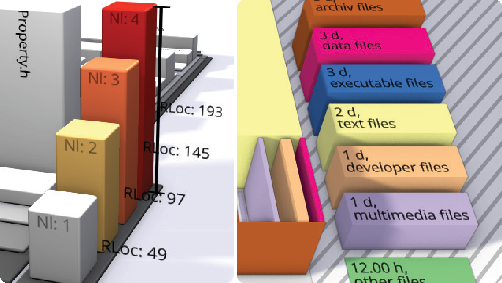
\includegraphics[width=\linewidth]{labeling-in-3d-legends}
	\vspace*{-1.0\baselineskip}
	\label{fig:legends}
\end{figure}
\noindent
This is a basic example of static label placement in 3D space. Contrary to 2D space, we cannot use pixel or point as a unit for font size and positioning, since the actual size of a label depends on its position and the position of the camera. Thus there is no purpose in using any unit other that world space coordinates for font size and positioning:

\lstinputlisting[language = TypeScript, label = lst:position3d]{listings/position3d.js}

\subsection{2D Projected Label at 3D Position}
\begin{figure}[h]
	\vspace*{-0.75\baselineskip}
	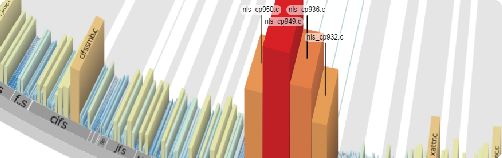
\includegraphics[width=\linewidth]{labeling-poles-adaptive}
	\vspace*{-1.0\baselineskip}
	\label{fig:lineLabel}
\end{figure}
\noindent
Projected 3D labels are positioned in 3D space, but projected onto a 2D plane. The model view projection is used to position the label based on its anchor point that is specified in world coordinates, while the label itself is treated as 2D:

\lstinputlisting[language = TypeScript, label = lst:projected3d]{listings/projected3d.js}

\subsection{Labeling along 3D Splines}
\begin{figure}[h] 
	\vspace*{-0.75\baselineskip}
	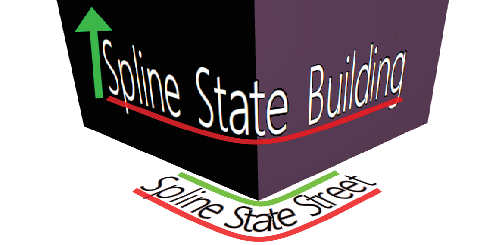
\includegraphics[width=\linewidth]{labeling-spline}
	\vspace*{-1.0\baselineskip}
	\label{fig:building3dspline}
\end{figure}
\noindent
Splines can be useful, e.g., for annotating a 3D-building by wrapping a label around the walls or for labeling a river.
A spline has several properties: control points, knot values and degree. Two of them must be given for defining the spline, the third can be calculated.
For every glyph on a spline, the same up vector can be used. However in 3D space, the up vector can also be different for every glyph. In addition to the base spline (that is the baseline in typesetting), a top spline is defined, which is used to calculate an up vector for every glyph. That up vector is defined by the position of the glyph on the base spline and the corresponding position on the top spline:

\lstinputlisting[language = TypeScript, label = lst:spline3d]{listings/spline3d.js}

\subsection{Adaptive Label Placement}
\noindent
To maintain readability for rendered glyphs, their placement should adapt to changes of view or occluding geometry. When annotating a point, the label can be placed at different angles; when annotating a line, the label can be written over any part of the line -- to mention a few scenarios. We address those issues with two examples, based on uses cases in Treemap-based software visualizations:\medskip

\subsubsection{Adaptive Label Placement in Screen Space}
\noindent
The first example shows an external label in screen space. It uses a line in world space to connect the label to the corresponding object. Changing the view might later result in changing the line origin and thus changing the label position.
\begin{figure}[h]
	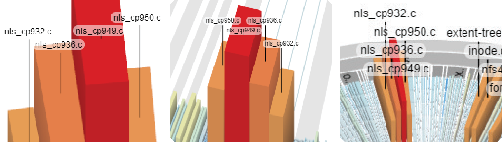
\includegraphics[width=\linewidth]{labeling-adaptive}
	\vspace*{-1.0\baselineskip}
	\label{fig:adaptiveLabelPlacement}
\end{figure}

\subsubsection{Adaptive Label Placement using a Box Proxy}
\begin{figure}[h]
	\vspace*{-0.75\baselineskip}	
	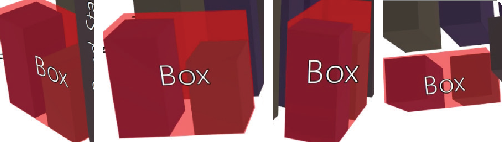
\includegraphics[width=\linewidth]{labeling-box-proxy}
	\vspace*{-1.0\baselineskip}
	\label{fig:boxRef}
\end{figure}
\noindent
The second example uses a proxy in form of a box. Different surfaces of the box are usable for the label's position. It also possible to change the direction and up vector of the label accordingly. At this point, a smart placement algorithm can be interposed to calculate the label's placement taking into account the proxy geometry, the current view, or occluding geometry:

\lstinputlisting[language = TypeScript, label = lst:proxygeom3d]{listings/proxygeom3d.js}

\subsection{Labeling with Level Of Detail} 
\begin{figure}[h]
	\vspace*{-0.75\baselineskip}
	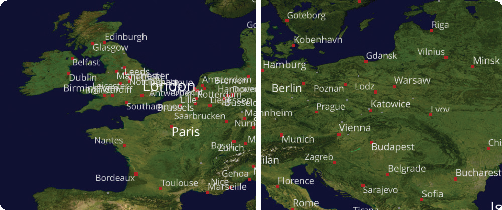
\includegraphics[width=\linewidth]{labeling-cloud-lod}
	\vspace*{-1.5\baselineskip}
	\label{fig:cloud}
\end{figure}
\noindent
When rendering a large amount of labels, the view is easily cluttered and labels overlap or occlude other objects. To prevent that, it is possible to choose a subset of all labels based on certain constraints, e.g., only the 20 most important labels (criterion: label priority or weight), a minimum font size (view-based in 3D), or only certain semantic groups that can have precedence for visual display over other groups.

The following example shows how to define such a label cloud, where multiple labels with the same positioning and stylization properties are gathered. Constraints of different types are added that are evaluated before the labels are rendered:

\lstinputlisting[language = TypeScript, label = lst:projected3d.multiple]{listings/projected3d.multiple.js}

